\documentclass[twoside,twocolumn]{article}
\usepackage{stackengine}
\usepackage{blindtext} 
\usepackage{amsmath}
\usepackage[sc]{mathpazo} 
\usepackage[T1]{fontenc} 
\linespread{1.05} 
\usepackage{microtype} 
\usepackage{amssymb}
\usepackage[italian]{babel} 
\usepackage{tikz}
\usepackage[hmarginratio=1:1,top=32mm,columnsep=20pt]{geometry} 
\usepackage[hang, small,labelfont=bf,up,textfont=it,up]{caption} 
\usepackage{booktabs} 
\usepackage{tocbibind}
\newtheorem{theorem}{Teorema}
\newtheorem{lemma}{Lemma}
\newcommand{\listofalgorithmes}{\tocfile{\listalgorithmcfname}{loa}}
\usepackage{lettrine} 
\usepackage{graphicx} 
\usepackage{enumitem} 
\setlist[itemize]{noitemsep} 
\usetikzlibrary{shapes.misc, positioning}
\usepackage{abstract} 
\renewcommand{\abstractnamefont}{\normalfont\bfseries}
\renewcommand{\abstracttextfont}{\normalfont\small\itshape} 
\usepackage{titlesec} 
\renewcommand\thesection{\Roman{section}} 
\renewcommand\thesubsection{\roman{subsection}} 
\newcommand{\notimplies}{%
	\mathrel{{\ooalign{\hidewidth$\not\phantom{=}$\hidewidth\cr$\implies$}}}}
\titleformat{\section}[block]{\large\scshape\centering}{\thesection.}{1em}{} 
\titleformat{\subsection}[block]{\large}{\thesubsection.}{1em}{}
\usepackage{fancyhdr} 
\pagestyle{fancy} 
\fancyhead{} 
\fancyfoot{} 
\fancyhead[C]{BetaReg $\bullet$ Applied Statistic and Data Analysis} % Custom header text
\fancyfoot[RO,LE]{\thepage} 

\usetikzlibrary{positioning}

\newcommand{\LivelloReale}{Livello reale}
\newcommand{\LivelloAstratto}{Livello astratto }
\newcommand{\qzero}{$q_0$}
\newcommand{\quno}{$q_1$}
\newcommand{\qdue}{$q_2$}
\newcommand{\qtre}{$q_3$}
\newcommand{\qzerohat}{$\hat{q_0}$}
\newcommand{\qunohat}{$\hat{q_1}$}
\newcommand{\yslant}{0.5}
\newcommand{\xslant}{-0.6}

\usepackage{titling}

\usepackage{hyperref} 

\usepackage{algorithm2e} %for psuedo code
 \SetKwProg{Fn}{function}{}{end-function}
  \SetKwProg{Try}{try}{}{}
  \SetKwProg{Catch}{catch}{}{end}
 \RestyleAlgo{boxed}
%\usepackage[lmargin=3.81cm,tmargin=2.54cm,rmargin=2.54cm,bmargin=2.52cm]{geometry}

\def\rlwd{.4pt}
\def\rlht{1.1pt}
\def\shatvrule{\rule{\rlwd}{\rlht}}
\def\shat#1{%
	\setbox0=\hbox{$#1$}%
	\stackon[0pt]{\stackon[1pt]{\ensuremath{#1}}{%
			\shatvrule\kern\wd0\kern-\rlwd\kern-\rlwd\shatvrule}}%
	{\rule{\wd0}{\rlwd}}%
}

\setlength{\droptitle}{-4\baselineskip} 

\pretitle{\begin{center}\Huge\bfseries} 
	\posttitle{\end{center}} 
\title{BetaReg: pacchetto R} 
\author{
	\textsc{Marta Rotari - Idriss Riouak} \\[1ex] 
	\normalsize Università degli studi di Udine \\ 
	\normalsize Dipartimento di matematica e informatica \\ 
	\normalsize Applied Statistic and Data Analysis\\
	\normalsize \href{mailto:idriss.riouak@spes.uniud.it}{idriss.riouak@spes.uniud.it} 
	\normalsize \href{mailto:marta.rotari@spes.uniud.it}{marta.rotari@spes.uniud.it} 
}
\date{\today} 
\renewcommand{\maketitlehookd}{%
	\begin{abstract}
		\noindent  La regressione è un metodo statistico che permette l'analisi delle relazioni che intercorrono tra due variabili che possono assumere valori nel continuo o nel discreto. Lo scopo di questa relazione è quello di studiare e analizzare un modello di regressione nel quale il dominio delle variabili di risposta possono assumere valori nell'intervallo limitato $(0,1)$.
		Il modello analizzato è chiamato modello di regressione con variabili di risposta Beta, introdotto per la prima volta nel 2004 da Cribari-Neto e Ferrari \cite{2004}. In particolare andremo ad analizzare l'implementazione in \emph{R} del modello, evidenziandone i pregi e difetti.
	\end{abstract}
}


\begin{document}
	

	\maketitle
	
	\section{Introduzione}
	Un modello di regressione è un modello statistico, il cui scopo è sia quello di studiare ed analizzare le relazioni tra una una variabile \emph{dipendente}, detta variabile di risposta, e una o più variabili \emph{indipendenti}, dette variabili esplicative, che di effettuare predizioni dato un nuovo valore per la variabile esplicativa.
	
	Il \emph{modello di regressione lineare semplice} ha la seguente forma
	\begin{equation}\label{eq:lrm}
		 y_i=\alpha + \beta x_i + \varepsilon_i 
	\end{equation}

	dove la componente casuale $\varepsilon_i$ è normalmente distribuita con media zero e varianza $\sigma^2$.
	Tale modello è ampiamente utilizzato in svariate applicazione, tuttavia non è appropriato per situazioni dove la variabile risposta è limitata ad assumere valori in un intervallo $(0,1)$, in quanto, i valori stimati potrebbero eccedere tale intervallo \footnote{Un esempio classico è <<Teaching Program>>\cite{PV}(pg. 67)}. Per ovviare a questo problema, prima dell'avvento del modello di regressione con variabili \textit{Beta}, la variabile di risposta $y$ veniva trasformata per poter assumere valori in$\mathbb{R}$, per esempio applicando$\tilde{y}=log(\frac{y}{1-y})$ alla quale veniva applicato il modello di regressione lineare semplice. Ma tale approccio presentava alcune problematiche come: I parametri venivano interpretati rispetto a $E[\tilde{y}]$ anziché rispetto a $E[y]$; le variabili casuali con valori nell'intervallo unitario sono tipicamente eteroschedastiche che causano la mancanza di alcune ipotesi fondamentali nel modello di regressione lineare (la varianza aumentava all'avvicinarsi della media e decresceva spostandosi verso i limiti dell'intervallo) ed infine l'asimmetria della distribuzione di tassi e di proporzioni dunque la stima degli intervalli per il test dell'ipotesi basate su approssimazioni Gaussiane portavano a grosse imprecisioni sopratutto in campioni di piccole dimensioni.

	Nel 2004, Cribari-Neto e Ferrari, con l'articolo \emph{"Beta Regression for Modelling Rates and Proportions"} \cite{2004}, propongono un nuovo modello di regressione per variabili continue con valori in $(0,1)$ come possono essere proporzioni e tassi, assumendo che la variabile risposta sia beta-distribuita. Successivamente nel 2016, nell'articolo \emph{``Beta Regression in R''} \cite{CNF}, i due autori forniscono un'implementazione in R di tale modello.
	
	\section{Beta distribuzione}
	Come già anticipato, il modello di regressione Beta si basa sull'ipotesi che la variabile risposta $y$ sia \textit{beta}-distribuita.
	La distribuzione Beta e una distribuzione di probabilità continua definita da due parametri $p$ e $q$ sul''intervallo unitario $[0,1]$. \footnote{Si noti che se la variabile $y$ dovesse assumere valori nell'intervallo $(a,b)$, dove $a < b$ e siano valori noti, allora è possibile modellare $\frac{y-a}{b-a}$ al posto di $y$. Mentre se la variabile $y$ dovesse assumere come valori in [0,1], una possibile trasformazione potrebbe essere $\frac{y\cdot (n-1) \cdot 0.5}{n}$ dove $n$ è la grandezza del campione.} Questa distribuzione governa la probabilità $p$ di un Processo di Bernoulli a posteriori dell'osservazione di $\alpha -1$ successi e $\beta -1$ insuccessi quando $p$  è a priori distribuita uniformemente tra $0$ e $1$. 
	
	La funzione densità di probabilità di una variabile casuale beta è data nel seguente modo:
	$$f(y;p,q)=\frac{\Gamma(p+q)}{\Gamma(p)\Gamma(q)}y^{p-1}(1-y)^{q-1},\ \ \ \ 0 <y<1$$ 
	Dove $p>0$ e $q>0$ e $\Gamma(\cdot)$ è la funzione gamma $\Gamma(z)=\int_{0}^{+ \infty} t^{z-1} e^{-t} dt.$ 
	
	\emph{Ferrari e Cribari-Neto} ne hanno proposto una parametrizzazione differente per il suo utilizzo nel modello:

	$$
		\hspace{-4mm}
	f(y,\mu,\phi)=\frac{\Gamma{\phi}}{\Gamma(\mu\phi)\Gamma((1-\mu)\phi)}y^{\mu\phi^{-1}}(1-y)^{(1-\mu)\phi-1} $$
	con 
	\begin{align*}
	\mu&=\frac{p}{p+q} \ , & \phi=p+q
	\end{align*}
	dove $0<\mu<1$, $\phi >0 $ e $0<y<1$. 
		\begin{figure}[h]
		\hspace*{-0.5cm}
		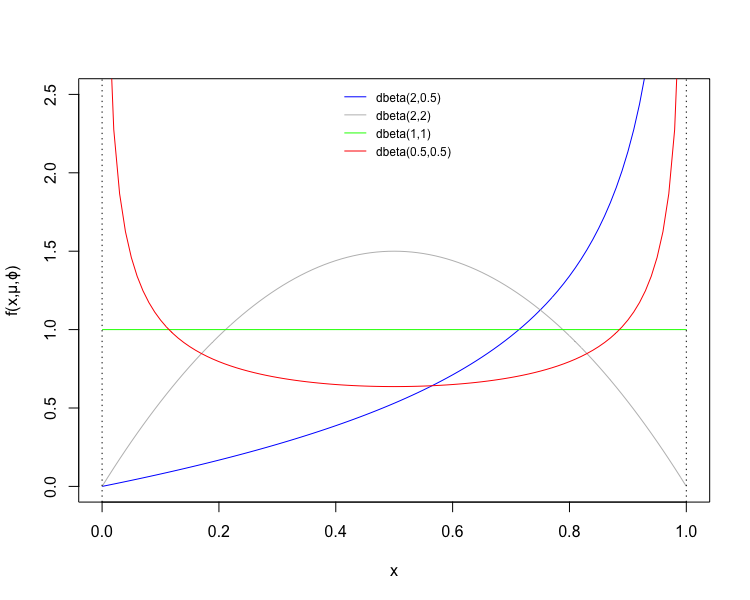
\includegraphics[scale=.3]{Beta}
		\caption{Rappresentazione grafica della distribuzione Beta, utilizzando il comando R: \emph{dbeta}.}
	\end{figure}
	
	
	
	Denoteremo con $y \sim \mathbb{\mathcal{B}}(\mu,\phi)$ se  la v.c. $y$ segue una beta distribuzione con parametri $\mu$ e $\phi$. Si noti che $p=\mu\phi$ e $q=\phi(1-\mu)$, da cui segue che $$E(y)=\mu \ \ e \ \ V(y)=\frac{V(\mu)}{1+\phi}=\frac{\mu(1-\mu)}{1+\phi}$$. 
	
	Il parametro $\phi$ è anche chiamato \emph{parametro di precisione}, in quanto per $\mu$ fissato, all'aumentare di $\phi$ diminuisce il valore della varianza.

\section{Il modello di regressione Beta}
Sia $y_1, y_2, ... ,y_n$ un campionamento casuale tale che $\forall_{i=1}^n: y_i \sim \mathbb{\mathcal{B}}(\mu_i, \phi)$. Il modello di regressione Beta è definito nel seguente modo
\begin{equation}g(\mu_i)=x_i^t\beta=\eta_i
\label{eq:mui}
\end{equation}
dove $\beta=(\beta_1, \beta_2, ..., \beta_k)^t$, con $k<n$, è un vettore $k \times 1$, $x_i=(x_{i1}, x_{i2},...,x_{ik})^t$ è un vettore di $k$ variabili esplicative, per convenzione $x_{i1}=1$ in tal modo ogni modello ha l'intercetta; mentre $\eta_i=\beta_1x_{i1}+...+\beta_kx_{ik}$ è un predittore lineare. Infine $g(\cdot):(0,1)\rightarrow\mathbb{R} \in \mathcal{C}^2$ è una funzione  di collegamento avente derivata seconda costante. Le funzioni di collegamento più utilizzate sono:
%%FIX-ME: Aggiungere commenti e dettagliare le funzioni di collegamento.
\begin{itemize}
	\item \textbf{logit:} $g(\mu)=log(\frac{\mu}{(1-\mu)}) $
	\item \textbf{probit:} $g(\mu)=\varPhi^{-1}(\mu)$, dove $\varPhi(\cdot)$ è la funzioni di distribuzione normale.
	\item \textbf{log-log complementare:}\\ $g(\mu)=\log(-\log(1-\mu))$
	\item \textbf{log-log:}$g(\mu)=\log(-\log(\mu))$
	\item \textbf{Cauchy:} $g(\mu)=\tan(\pi(\mu-0.5))$
\end{itemize}

Denotiamo con $l(\beta,\phi)=\sum_{i=1}^{n}l_i(\mu_i,\phi)$ la funzione di verso somiglianza, dove 
\begin{align*}
l_i(\mu_i, \phi)=&\log \Gamma(\phi)-\log (\mu_i\phi)\\
&-\log\Gamma((1-\mu_i)\phi)+(\mu_i\phi-1)\log y_i \\&
+  \{(1-\mu_i)\phi -1 \}\log(1-y_i)
\end{align*}
con $\mu_i$ definito come nell'equazione \eqref{eq:mui} ovvero $\mu_i=g^{-1}(x_i^t\beta)$.

	\subsection{Determinizzazione degli stimatori.}
%%FIX-ME: determinare qual'è l'intervallo di t di \mu e y.
Siano$$y_t^*=log(\frac{y_t}{1-y_t})$$ e $$\mu_t^*=\psi(\mu_t\phi)-\psi((1-\mu_t)\phi),$$ dove $\psi(x)=\frac{\partial \log \Gamma(x)}{\partial x}$ con $x>0$ è detta funzione \emph{digamma.} Denotiamo con $$\nabla(\beta,\phi)=\begin{pmatrix}
U_\beta(\beta,\phi)\\U_\phi(\beta,\phi)
\end{pmatrix}$$
la funzione \emph{score}, ottenuta differenziando la funzione di log-verosimiglianza rispetto i due parametri sconosciuti. Dunque 
$$U_\beta(\beta,\phi)=\frac{\partial l(\beta,\phi)}{\partial \beta}=\phi X^tT(y^*-u^*), $$
dove $X$ è la matrice del modello di dimensione $n \times k$, $T$ è una matrice diagonale la cui dimensione $n \times n$ definita come $T=diag\{g'(\mu)_1^{-1},...,g'(\mu_i)^{-1}\}$, $y^*=(y_1^*, ..., y_n^*)$ e $\mu^*=(\mu_1^*, ..., \mu_n^*)$. Mentre \begin{align*}
U_\phi(\beta,\phi)=&\sum_{t=1}^{n}\{ \mu_t(y_t^*-\mu_t^*)
+ log(1-y_t)\\ & - \phi((1-\mu_t)\psi)+ \phi(\psi)  \}
\end{align*}
Possiamo dunque concludere che gli stimatori di massima verosimiglianza (MLEs) per $\beta$ e $\phi$ sono ottenibili ponendo rispettivamente $U_\beta(\beta,\phi)$ e $U_\phi(\beta,\phi)$ uguali a zero.
Tale tipo di equazioni non sono risolvibili analiticamente, ma il risultato può essere approssimato attraverso un  algoritmo numerico quale l'algoritmo di \emph{Newton}. Tali algoritmi necessitano di un punto di partenza ($\beta_0,\phi_0$), che nel caso di $\beta$ utilizzando il metodo dei minimi quadrati è $$ \beta_0=(X^tX)^{-1}X^tz,$$ dove  $z=(g(y_1),...,g(y_n))^t$.
Mentre per $\phi$, \emph{Ferrari e Cribari-Neto} in \cite{2004} suggeriscono  come punto di partenza $$
\phi_0=\frac{1}{n}\sum_{t=1}^{n}\frac{\breve{\mu}_t(1-l\breve{\mu}_t)}{\breve{\sigma}_t^2},
$$
dove $\breve{\mu}_t$ è ottenuto applicando la funzione $g^{-1}(\cdot)$ al \emph{t-esimo} valore stimato dal modello di regressione lineare di $g(y_1),...,g(y_n)$ su $X$: $$\breve{\mu}_t=g^{-1}(x_t^t(X^tX)^{-1}X^t z)$$  e $$ \breve{\sigma}_t^2=\frac{\breve{e}^t\breve{e}}{(n-k)[g'(\breve{\mu})_t]^2} $$
dove $\breve{e}=z-X(X^tX)^{-1}X^tz$.

Consideriamo ora la matrice d'informazione di \emph{Fisher}, che servirà per poter approssimare l'errore standard degli stimatori $\hat{\beta}$ e $\hat{\phi}$. Poniamo prima $W=diag\{w_1,...,w_n\}$, con $$w_t=\phi\{\psi'(\mu_t\phi)+ \psi'((1-\mu_t)\phi) \}\frac{1}{\{g'(\mu_t)\}^2}, $$ $c=(c_1,...,c_n)^t$,  dove $$c_t=\phi\{\psi'(\mu_t\phi)\mu_t-\phi'((1-\mu_t)\phi)(1-\mu_t) \}$$
e $\psi'(\cdot)$ è la funzione \emph{trigamma}, definita come segue $$\psi'(x)=\frac{\partial^2}{\partial z^2}\log \Gamma(x).$$
Sia dunque $K$ la matrice d'informazione di \emph{Fisher}:

\begin{equation}
 K = K(\beta,\phi) =
 	 \begin{pmatrix} 
 	 	K_{\beta\beta} & K_{\beta\phi}\\
 	 	K_{\phi\beta} & K_{\phi\phi} 
 	 \end{pmatrix}, 
 	 \label{eq:Fisher}
\end{equation}
dove 
\begin{itemize}
	\item $K_{\beta\beta}=\phi X^tWX$,
	\item $K_{\beta\phi}=K_{\phi_\beta}^t=X^tTc$,
	\item $K_{\phi \phi}=tr(D)$.
\end{itemize}

Sotto le condizioni di normalità, d'indipendenza e di omogeneità di varianza delle variabili, quando la grandezza del campione è grande, vale che
$$ \begin{pmatrix}\hat{\beta}\\ \hat{\phi} \end{pmatrix} \sim \mathcal{N}_{k+1}\Bigg(\begin{pmatrix}\beta\\ \phi \end{pmatrix},K^{-1}\Bigg).$$ 

Denoteremo con $SE(\hat{\beta_j})$ l'errore standard asintottico del MLE $\hat{\beta_j}$, che si ottiene dall'inversa della matrice di \emph{Fisher} \eqref{eq:Fisher} valutata in $\hat{\beta_j}$ e in $\hat{\phi}$.

\subsection{Intervallo di confidenza}
E' possibile determinare un intervallo di confidenza $(1-\alpha)100\%$\footnote{con $\alpha \in (0,\frac{1}{2})$.} per i coefficienti $\hat{\beta}_j$, con $j=1,...,k$. Tale intervallo è:
$$ \bigg[\hat{\beta_j} \pm \Phi^{-1}\bigg(1-\frac{\alpha}{2}SE(\hat{\beta_j})\bigg)\bigg], $$
dove $\Phi(\cdot)$ è la funzione di distribuzione cumulativa di una variabile casuale normale. 

Analogamente un intervallo di confidenza $(1-\alpha)100\%$ per il parametro $\hat{\phi}$ è il seguente
$$\bigg[\hat{\phi} \pm \Phi^{-1}\bigg(1-\frac{\alpha}{2}SE(\hat{\phi})\bigg)  \bigg] $$ dove 
\begin{align*}
SE(\hat{\phi})&=\sqrt{tr(D)-\phi^{-1}c^tT^tX(X^tWX)^{-1}X^tTc}\\
&=\sqrt{\hat{\gamma}}.
\end{align*}

In fine è possibile determinare un intervallo di confidenza $(1-\alpha)100\%$ per il valore atteso della variabile risposta $\mu$ per un dato vettore d'osservazioni delle variabili regressori $x_0=[1,x_{01},x_{02},...,x_{0k}]$:
$$[Lim_{sx}, Lim_{dx}]\footnote{Tale intervallo è valido solo per funzioni di collegamento $g(\cdot)$ strettamente crescenti.}$$ dove 
$$Lim_{sx}=\bigg[ g^{-1}\bigg(\hat{\eta} -\Phi^{-1}\Big(\frac{1-\alpha}{2}\Big)SE(\hat{\eta})\bigg)  \bigg]  $$
mentre
$$ Lim_{dx}=\bigg[ g^{-1}\bigg(\hat{\eta} +\Phi^{-1}\Big(\frac{1-\alpha}{2}\Big)SE(\hat{\eta})\bigg)  \bigg], $$
con $\hat{\eta}=x_0^t \hat{\beta}$ e $SE(\hat{\eta})=\sqrt{x_0^t \widehat{\text{cov}}(\hat{\beta})x_0}$ dove $\widehat{\text{cov}}(\hat{\beta})$ è ottenuto dall'inversa della matrice di \emph{Fisher} \eqref{eq:Fisher} valutata negli MLEs escludendo la riga e la colonna relative al parametro di precisione $\hat{\phi}$.
\newpage
\tableofcontents
		\begin{thebibliography}{99} 
	\bibitem{2004} \textbf{Beta Regression for Modelling Rates and Proportions.}, Ferrari SLP, Cribari-Neto Francisco (2004).  Journal of Applied Statistics, 31(7), 799–815.
	\bibitem{CNF} \textbf{Beta Regression in R}, Francisco Cribari-Neto, Achim Zeileis.\\
	\bibitem{PV} \textbf{Towards multiple linear regression and logistic regression}, Paolo Vidoni, 2017-2018. Lecture 5. Applied Statistics and Data Analysis.
	\end{thebibliography}

\end{document}